\subsection{Dati e risultati}

L'oscillatore a ponte di Wien (figura \ref{fig:circ8}), che prende il nome dal fatto che non è altro
che un ponte di wien modificato con l'inserimento di un amplificatore operazionale, è un particolare
tipo di oscillatore che genera onde sinusoidali. È evidente che un oscillatore deve avere un
feedback positivo, altrimenti non è caratterizzato dall'instabilità tipica di un oscillatore.

\paragraph{Principio di funzionamento.}

All'accensione dell'alimentazione, l'operazionale ha l'uscita ad una tensione $V\ped{out}$ diversa da zero,
spesso in saturazione positiva o negativa. Questo è dovuto alla tensione di offset e al rumore ed è il trigger
che fa partire l'oscillatore. Trascuriamo per un momento la presenza della lampadina.

L'improvviso passaggio da zero a $V\ped{out}$ alla accensione è un segnale che può essere immaginato come
uno scalino e che quindi ha uno spettro in frequenza molto ampio. Per comprendere il funzionamento dell'oscillatore
è quindi necessario studiare il partitore formato da $R_2$, $R_3$, $C_1$ e $C_2$ e vedere come si comporta
in frequenza. La funzione di trasferimento del partitore è ($R = R_2 = R_3$, $C = C_1 = C_2$)

\begin{equation}
    H(s) = \frac{\left(\frac{1}{R} + sC\right)^{-1}}{\left(sC + \frac{1}{R}\right)^{-1} + R + \frac{1}{sC}}
\end{equation}
%
che una volta semplificata un po' prende la forma

\begin{figure}[b!]
    \begin{circuitikz}[scale=0.85, transform shape]
        \draw
            (0, 4) node[rground] {}
            to [C, l=$C_1$ 15 nF] (0, 6)
            to (1, 6)
            to [R, l=$R_3\;10 \si{\kilo\ohm}$] (1, 4)
            node[rground] {}
            (1, 6) to [R, l=$R_2\;10\si{\kilo\ohm}$] (1, 8)
            to [C, l=$C_2$ 15 nF] (6.5, 8)
            to (6.5, 3)
            to [vR, l=$R_V\;1\si{\kilo\ohm}$] (3, 3)
            (5, 5.5) node[op amp, yscale=-1] (opamp) {} 
            (1, 6) to (opamp.+)
            (opamp.-) to (3, 5) to[short, -o] (3, 3)
            node[anchor=east] {$V^-$}
            to [R, l_=$R_1\;47\si{\ohm}$] (3, 1)
            to [lamp, l=12 V 50 mA] (3, 0)
            node[rground] {}
            (opamp.out) to[short, -o] (7, 5.5)
            node[anchor=west] {$V\ped{out}$}
            (opamp.up) to [short, -o] ++(0, -0.5) node[below] {$-V\ped{cc}$}
            (opamp.down) to [short, -o] ++(0, .5) node[above] {$+V\ped{cc}$}
        ;
    \end{circuitikz}
    \caption{Oscillatore a ponte di Wien.}
    \label{fig:circ8}
\end{figure}

\begin{equation}
    H(s) = \frac{sRC}{1 + 3sRC + (sRC)^2}
\end{equation}

Nel dominio delle frequenze ($s = i\omega$) si ottiene il guadagno

\begin{equation}
    G = |H(\omega)| = \frac{\omega RC}{\sqrt{(1 - \omega^2R^2C^2)^2 + 9\omega^2R^2C^2}}
\end{equation}

Il grafico del guadagno è riportato in figura \ref{fig:partitore8}. Il massimo del guadagno si ha alla frequenza
angolare $\omega = 1/RC$ o per $f = 2\pi/RC \simeq \SI{42}{\kilo\hertz}$, dove il guadagno vale $1/3$. In pratica il partitore
si comporta come un filtro passa banda di primo ordine con un'attenuazione al di fuori delle frequenze di taglio
di -20 dB/decade.

\begin{figure}
    \centering
    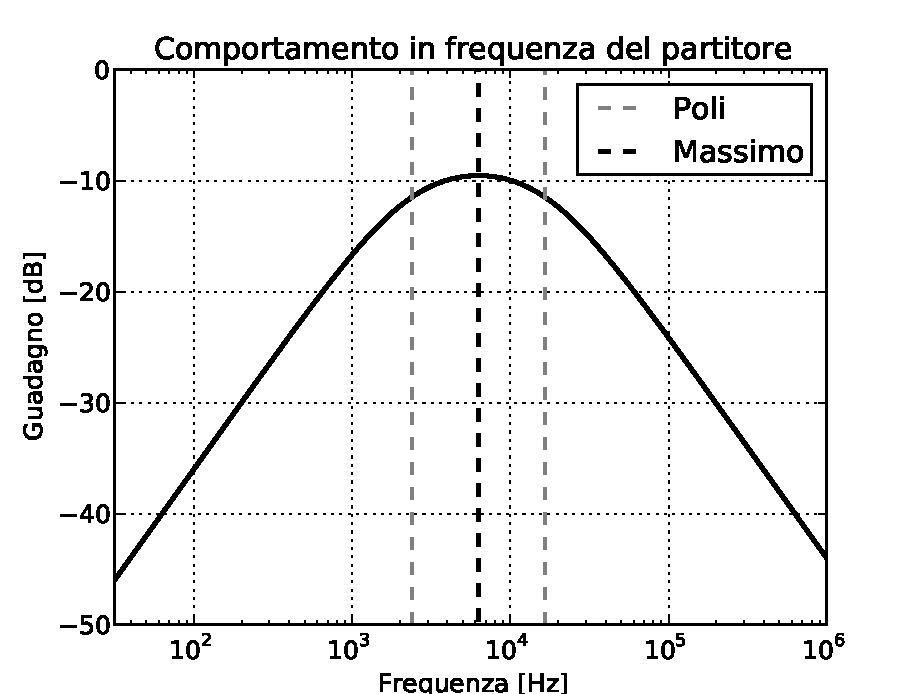
\includegraphics[width=\columnwidth]{figure/ctp.pdf}
    \caption{Comportamento in frequenza del partitore. Alla frequenza di picco il guadagno è esattamente 1/3.}
    \label{fig:partitore8}
\end{figure}

È quindi evidente che delle frequenze presenti nello ``scalino'' dopo l'accensione, alcune saranno più presenti
all'ingresso non-invertente dell'operazionale a causa di questo filtro. Le frequenze che vengono passate più facilmente,
sono attorno ai 42 kHz, vengono ridotte di un terzo.

Poiché l'operazionale ha anche un altro ramo di feedback negativo, l'operazionale tenderà ad aggiustare $V\ped{out}$
in modo che $V^-$ sia una replica di $v^+$. In questo caso significa che $V\ped{out}$ conterrà la stessa proporzione
delle frequenze presenti all'ingresso $V^+$, poiché il ramo di retroazione negativa è puramente resistivo e non filtra
le frequenze.

A questo punto il ``ciclo'' ricomincia, poiché all'ingresso non invertente giunge una versione filtrata di $V\ped{out}$.
Il sistema tende ad attenuare di molto le frequenze molto distanti dal picco a 42 kHZ, ma avendo un guadagno di 1/3 tende
ad attenuare anche le frequenze di picco. È evidente che se sul ramo di retroazione negativa il guadagno fosse esattamente 3
in modo da compensare il guadagno 1/3 sull'altro ramo,
si avrebbe che tutte le frequenze tranne quella centrale vengono rimosse, mentre quella centrale rimane inalterata.
Si ottiene così un onda sinusoidale. È importante sottolineare che, anche se è stato presentato come un ciclo che si ripete,
il funzionamento del circuito è dinamico e avviene tutto allo stesso tempo.

È chiaro che deve esserci una perfetta cancellazione dei guadagni per ottenere l'oscillatore che vogliamo, poiché
se il guadagno complessivo fosse minore di 1, si avrebbe che il sistema ``va a zero'' oscillando, mentre se il guadagno
fosse maggiore di 1 il sistema si porterebbe rapidamente in saturazione. Ottenere questo matching è praticamente impossibile
e anche se si riuscisse ad ottenerlo sicuramente durerebbe poco, a causa dei coefficienti termici dei vari componenti.

\begin{figure}[b!]
    \centering
    \begin{circuitikz}
        \draw
            (0, 0) node[rground] {}
            to (0, 1) to (1, 1)
            to [R, l_=$R_2$] (1, 3)
            to (0, 3) to (0, 4) to (1, 4)
            to [R, l_=$R_1$] (1, 6)
            to (0, 6)
            to [short, -o] (0, 7)
            node[anchor=east] {$V\ped{in}$}
            (0, 1)
            to (-1, 1)
            to [C, l=$C_2$] (-1, 3)
            to (0, 3)
            (0, 4)
            to (-1, 4)
            to [C, l=$C_1$] (-1, 6)
            to (0, 6)
            (0, 3.5)
            to [short, -o] (2, 3.5)
            node[anchor=west] {$V\ped{out}$}
        ;
        \draw [decorate,decoration={brace,amplitude=10pt},xshift=-4pt,yshift=0pt]
            (-2, 0.5) -- (-2, 3.4) node [black,rotate=90,midway,yshift=0.7cm] 
            {\small Oscilloscopio}
        ;
        \draw [decorate,decoration={brace,amplitude=10pt},xshift=-4pt,yshift=0pt]
            (-2, 3.6) -- (-2, 6.5) node [black,rotate=90,midway,yshift=0.7cm] 
            {\small Sonda}
        ;
    \end{circuitikz}
    \caption{Schema circuitale del sistema oscilloscopio + sonda. Il nostro oscilloscopio riporta
        i dati $R_2 = 1$ \si{\mega\ohm} e $C_2 = 12$ pF.}
    \label{fig:circ_sonda8}
\end{figure}

Esistono varie soluzioni a questo problema, la più semplice delle quali è la seguente: invece di impostare un guadagno fisso
mediante una resistenza nella retroazione negativa si inserisce un componente, per esempio una lampadina, che varia la propria resistenza in base alla
corrente che scorre al suo interno. Usando una lampadina si otterrà un guadagno variabile. La lampadina va posta tra l'ingresso non invertente e
il riferimento Il guadagno diminuisce quando passa
molta corrente (poiché la resistenza aumenta con la corrente), ovvero quando il guadagno era più alto di 1, perché il segnale tende
ad andare in saturazione, aumentando la d.d.p. ai capi della lampadina. Al contrario, quando il guadagno è inferiore a 1 il segnale
tende a diminuire, diminuendo la corrente (e quindi la resistenza) e aumentando quindi i guadagno. È una sorta di feedback.

\begin{figure}[b!]
    \centering
    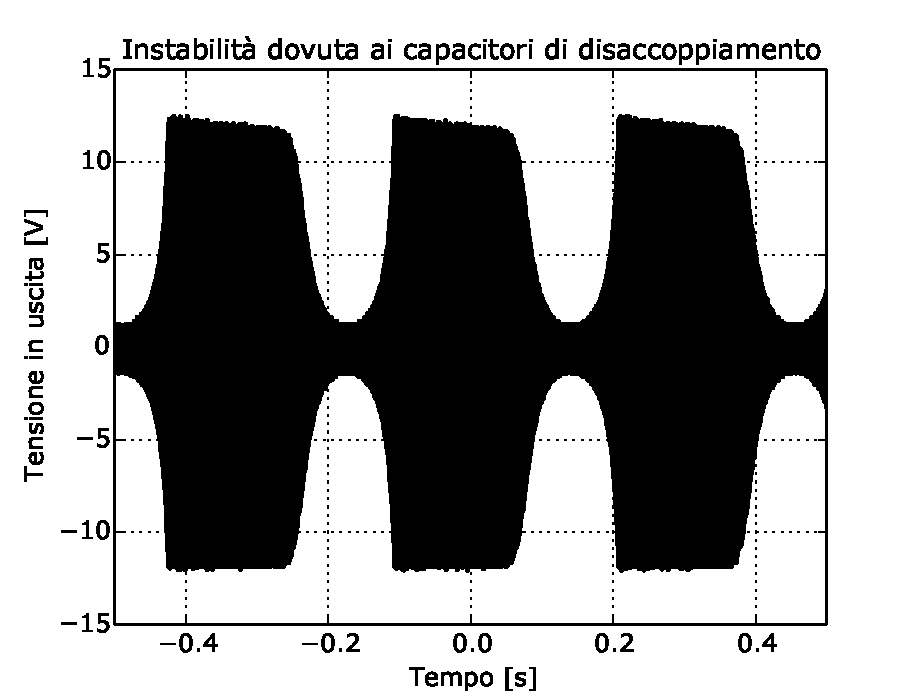
\includegraphics[width=\columnwidth]{figure/inststab.pdf}
    \caption{}
    \label{fig:instabilita8}
\end{figure}

In pratica si sfrutta l'inerzia della lampadina per attenuare le oscillazioni non volute del sistema. Con questo trucco
l'oscillatore diventa stabile ed è utilizzabile. La resistenza $R_1$ serve soltanto come limitatore di corrente.
La variazione della resistenza della lampadina è dovuta a effetti termici.

\begin{figure*}[b!]
    \centering
    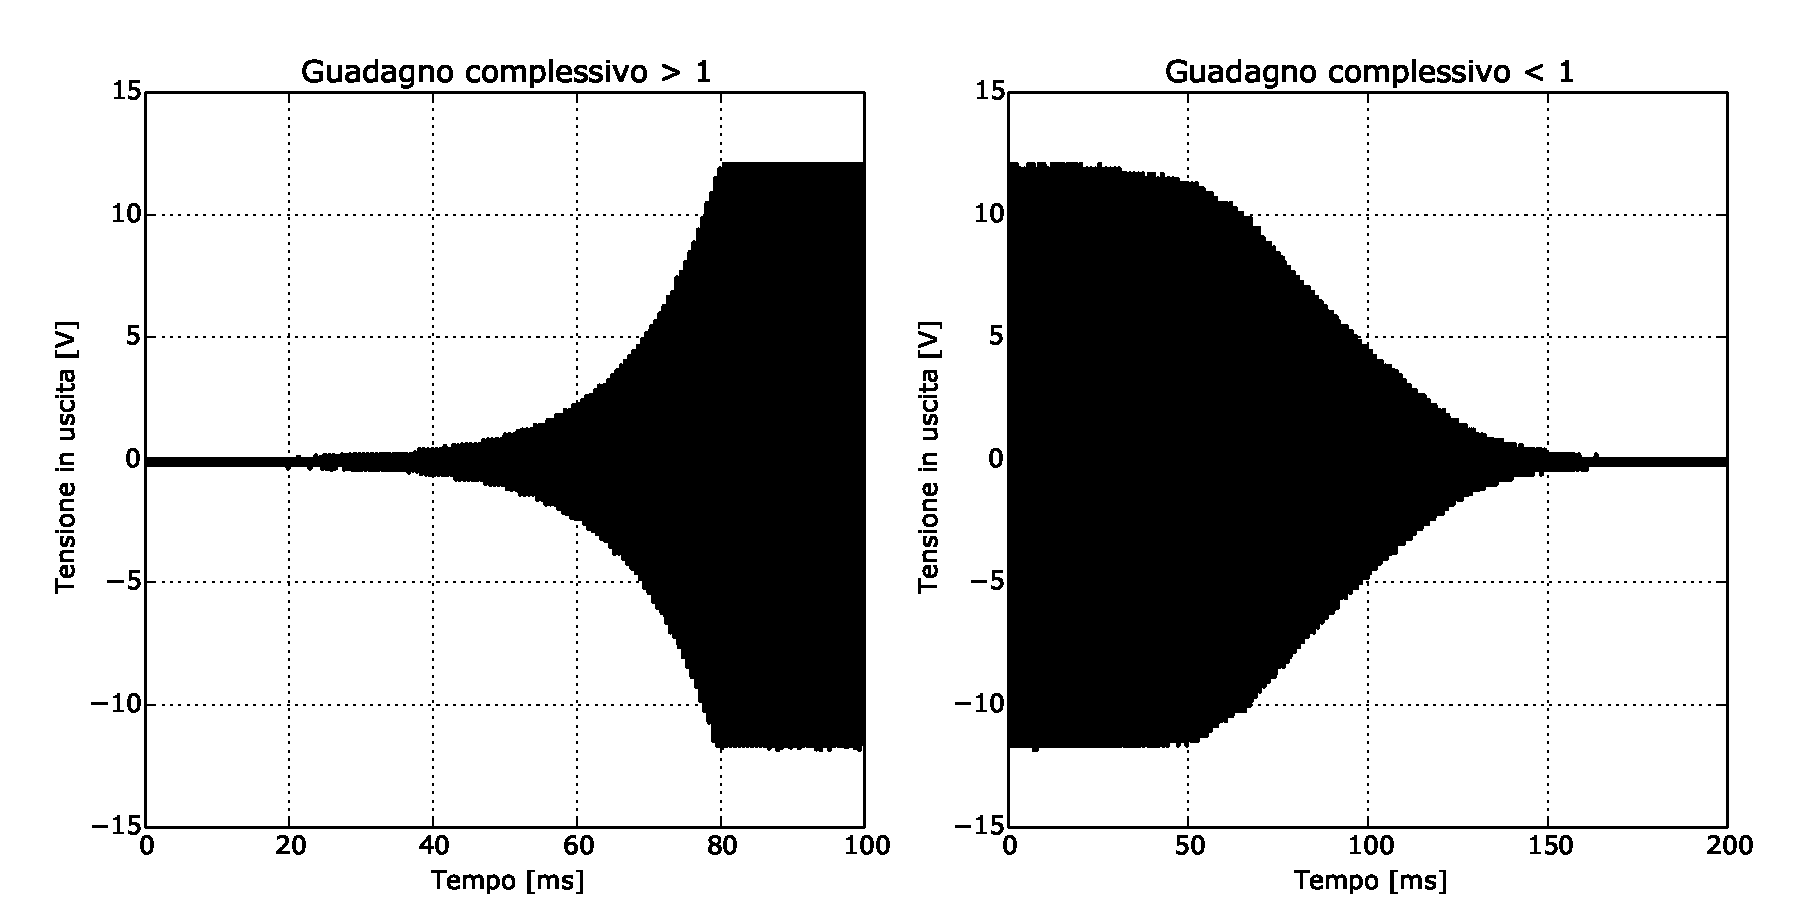
\includegraphics[width=\textwidth]{figure/exp_imp.pdf}
    \caption{Se la lampadina è assente il sistema è instabile e tende ad andare a zero (grafico a destra) oppure
        ad entrare in saturazione (immagine a sinistra). Nel caso di guadagno maggiore di 1 è evidente che l'operazionale entra in saturazione a circa
        12 V. L'immagine riporta solo la modulante del segnale. Ingrandendo l'immagine è possibile vedere che il segnale modulante
        contiene un onda sinusoidale.}
    \label{fig:exp_imp8}
\end{figure*}

\paragraph{Test del funzionamento.}

Inizialmente abbiamo montato il circuito senza inserire la lampadina. Abbiamo inserito un potenziometro nel ramo di feedback negativo
e la lampadina è stata sostituita con una resistenza da 220 \si{\ohm}. Abbiamo tentato, ovviamente senza successo, di eseguire
un matching dei guadagni. La figura \ref{fig:exp_imp8} riporta un paio di risultati in cui il segnale satura o va a zero a causa
del matching imperfetto dei guadagni. Il tempo impiegato dal sistema per saturare o per andare a riferimento è di poche decine
di millisecondi.

\begin{figure*}
    \centering
    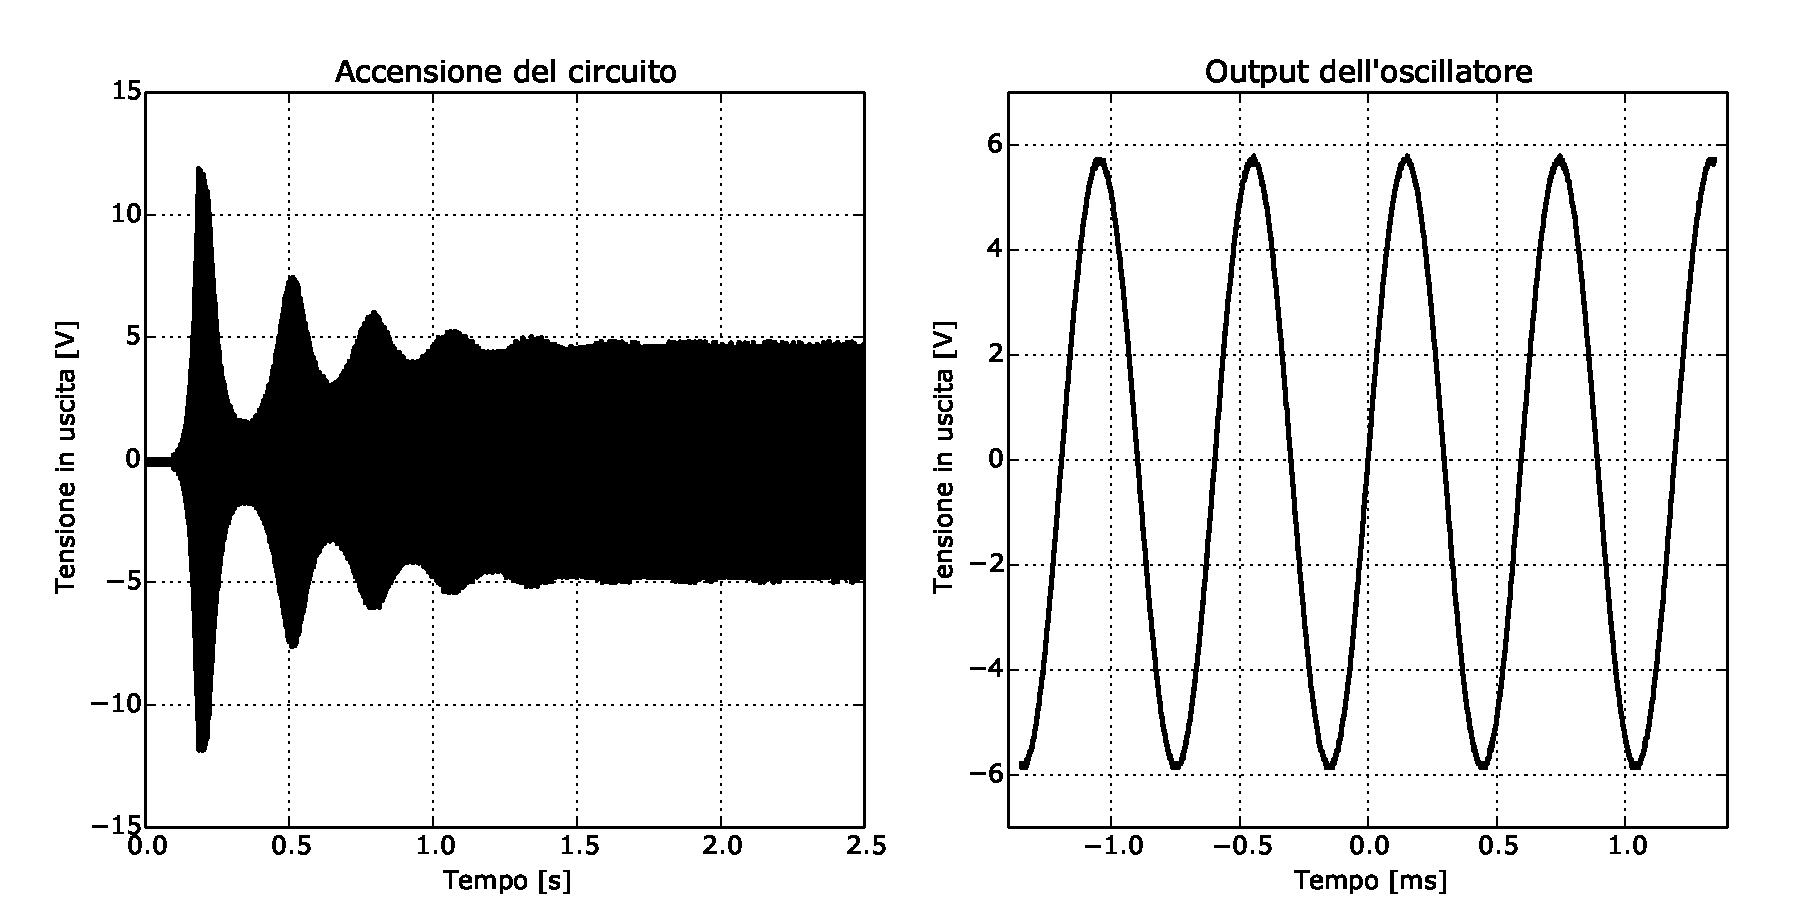
\includegraphics[width=\textwidth]{figure/stab.pdf}
    \caption{Nella figura a sinistra è mostrato il segnale modulante all'accensione del circuito. Il sistema oscilla ma a causa dell'inerzia della
        lampadina, dopo circa 2 secondi diventa stabile. L'ampiezza delle oscillazioni si riduce sempre di più. Nel grafico a destra è invece mostrato
        l'output dell'oscillatore una volta che si è stabilizzato. L'output è una sinusoide ed ha una frequenza di 1675 $\pm$ 5 Hz.}
    \label{fig:stab8}
\end{figure*}

Successivamente abbiamo inserito la lampadina, sempre mantenendo il trimmer per poter tarare il circuito. In questo caso l'oscillatore
si è rivelato stabile. La figura \ref{fig:stab8} mostra la tensione $V\ped{out}$ all'accensione e durante il funzionamento a regime dell'oscillatore.

Abbiamo inoltre provato ad inserire dei condensatori di disaccoppiamento sull'alimentazione dell'operazionale, notando che
l'output diventava instabile, producendo una sinusoide a tratti stabile e a tratti di ampiezza variabile.
Il passaggio tra i tratti di stabilità ed instabilità era periodico di periodo circa 0.3 secondi ed e riportato in figura \ref{fig:instabilita8}.

\paragraph{Compensazione delle sonde.}

Oltre alla costruzione dell'oscillatore, abbiamo anche compensato una sonda di misura. Ma vediamo la regione per cui
in alcuni casi è necessario utilizzare sonde che prevedono la possibilità di aggiustare la capacità interna.

In figura \ref{fig:circ_sonda8} è riportato uno schema di un oscilloscopio con collegata una generica sonda.
La sonda, non essendo un conduttore ideale, presenta una certa resistenza e possiede una capacità propria, causata
dal rumore di rete, dalle trasmissioni elettromagnetiche, ma anche dalla posizione del cavo rispetto ad altri conduttori.
L'ingresso dell'oscilloscopio presenta una capacità ed una resistenza, come tutti i circuiti elettrici.

È immediato comprendere che si forma un partitore, la cui tensione di uscita, contenendo delle capacità, dipende anche dalla
frequenza. All'ingresso dell'oscilloscopio abbiamo quindi un segnale diverso da quello che volevamo misurare ed inoltre non
è semplicemente un segnale ridotto di ampiezza (come accadrebbe se il partitore fosse solamente resistivo),
bensì un segnale storpiato. In taluni casi questo fatto non è accettabile e provoca errori nelle misure.
Vengono quindi in nostro aiuto le sonde compensate, ovvero sonde che permettono, attraverso una vite posta sul
puntale della stessa, di cambiare la capacità interna $C_1$.

Consideriamo la funzione di trasferimento del circuito in figura \ref{fig:circ_sonda8}:

\begin{equation}
    H(s) = \frac{Z_2}{Z_1 + Z_2} = \left(1 + \frac{R_1(sC_2R_2 + 1)}{R_2(sC_1R_1 + 1)}\right)^{-1}
\end{equation}

Si vede subito da questa formula che se $R_1C_1 = R_2C_2$ la frazione si riduce a $R_1/R_2$.
In questo caso la funzione di trasferimento dipende solo dalle resistenze, è indipendente dalla frequenza ($s = i\omega$)
e quindi il segnale non cambia forma. Agendo sulla vite di regolazione è possibile variare la capacità $C_1$
finché la relazione sopra non risulta soddisfatta, eliminando quindi l'effetto delle capacità.

\begin{figure}[t!]
    \centering
    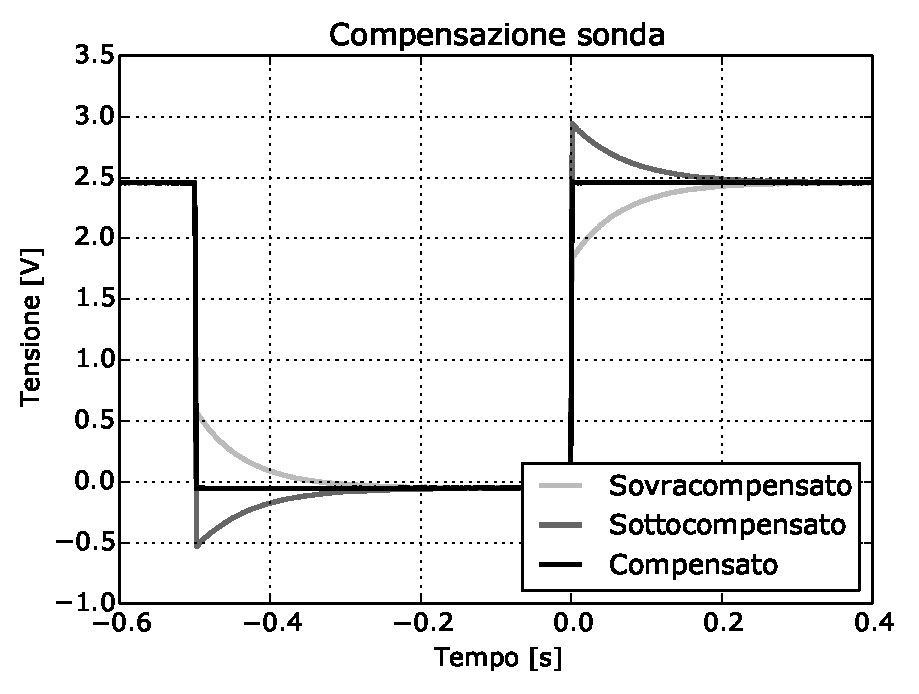
\includegraphics[width=\columnwidth]{figure/comp.pdf}
    \caption{Input dell'oscilloscopio con una sonda compensabile. Cambiando capacità
        si può ottenere una sottocompensazione, una sovracompensazione oppure compensare perfettamente
        le capacità, ottenendo un'onda quadra.}
    \label{fig:compensazione8}
\end{figure}

Nella pratica la compensazione viene fatta collegando la sonda al generatore di funzioni d'onda interno dell'oscilloscopio
e fornendo un'onda quadra. Sull'oscilloscopio si visualizzano l'onda quadra generata e l'ingresso proveniente dalla sonda.
Poiché prima della compensazione il partitore dipende dalla frequenza, all'ingresso non arriverà un'onda quadra ma un
segnale diverso, come quello in figura \ref{fig:compensazione8}. Agendo sulla vite si tenta quindi di trasformare il
segnale in ingresso in un onda quadra. La figura \ref{fig:compensazione8}, mostra cosa si riesce ad ottenere compensando
la sonda.

La procedura di compensazione è molto semplice e non ha creato alcun problema.

